% Options for packages loaded elsewhere
\PassOptionsToPackage{unicode}{hyperref}
\PassOptionsToPackage{hyphens}{url}
%
\documentclass[
  11pt,
  ignorenonframetext,
]{beamer}
\usepackage{pgfpages}
\setbeamertemplate{caption}[numbered]
\setbeamertemplate{caption label separator}{: }
\setbeamercolor{caption name}{fg=normal text.fg}
\beamertemplatenavigationsymbolsempty
% Prevent slide breaks in the middle of a paragraph
\widowpenalties 1 10000
\raggedbottom
\setbeamertemplate{part page}{
  \centering
  \begin{beamercolorbox}[sep=16pt,center]{part title}
    \usebeamerfont{part title}\insertpart\par
  \end{beamercolorbox}
}
\setbeamertemplate{section page}{
  \centering
  \begin{beamercolorbox}[sep=12pt,center]{part title}
    \usebeamerfont{section title}\insertsection\par
  \end{beamercolorbox}
}
\setbeamertemplate{subsection page}{
  \centering
  \begin{beamercolorbox}[sep=8pt,center]{part title}
    \usebeamerfont{subsection title}\insertsubsection\par
  \end{beamercolorbox}
}
\AtBeginPart{
  \frame{\partpage}
}
\AtBeginSection{
  \ifbibliography
  \else
    \frame{\sectionpage}
  \fi
}
\AtBeginSubsection{
  \frame{\subsectionpage}
}
\usepackage{amsmath,amssymb}
\usepackage{iftex}
\ifPDFTeX
  \usepackage[T1]{fontenc}
  \usepackage[utf8]{inputenc}
  \usepackage{textcomp} % provide euro and other symbols
\else % if luatex or xetex
  \usepackage{unicode-math} % this also loads fontspec
  \defaultfontfeatures{Scale=MatchLowercase}
  \defaultfontfeatures[\rmfamily]{Ligatures=TeX,Scale=1}
\fi
\usepackage{lmodern}
\usetheme[]{Madrid}
\usecolortheme{dolphin}
\usefonttheme{professionalfonts}
\usefonttheme{serif} % use mainfont rather than sansfont for slide text
\ifPDFTeX\else
  % xetex/luatex font selection
    \setmainfont[]{Arial}
\fi
% Use upquote if available, for straight quotes in verbatim environments
\IfFileExists{upquote.sty}{\usepackage{upquote}}{}
\IfFileExists{microtype.sty}{% use microtype if available
  \usepackage[]{microtype}
  \UseMicrotypeSet[protrusion]{basicmath} % disable protrusion for tt fonts
}{}
\makeatletter
\@ifundefined{KOMAClassName}{% if non-KOMA class
  \IfFileExists{parskip.sty}{%
    \usepackage{parskip}
  }{% else
    \setlength{\parindent}{0pt}
    \setlength{\parskip}{6pt plus 2pt minus 1pt}}
}{% if KOMA class
  \KOMAoptions{parskip=half}}
\makeatother
\usepackage{xcolor}
\newif\ifbibliography
\usepackage{graphicx}
\makeatletter
\def\maxwidth{\ifdim\Gin@nat@width>\linewidth\linewidth\else\Gin@nat@width\fi}
\def\maxheight{\ifdim\Gin@nat@height>\textheight\textheight\else\Gin@nat@height\fi}
\makeatother
% Scale images if necessary, so that they will not overflow the page
% margins by default, and it is still possible to overwrite the defaults
% using explicit options in \includegraphics[width, height, ...]{}
\setkeys{Gin}{width=\maxwidth,height=\maxheight,keepaspectratio}
% Set default figure placement to htbp
\makeatletter
\def\fps@figure{htbp}
\makeatother
\setlength{\emergencystretch}{3em} % prevent overfull lines
\providecommand{\tightlist}{%
  \setlength{\itemsep}{0pt}\setlength{\parskip}{0pt}}
\setcounter{secnumdepth}{-\maxdimen} % remove section numbering
\setbeamertemplate{footline}[frame number]
\ifLuaTeX
  \usepackage{selnolig}  % disable illegal ligatures
\fi
\usepackage{bookmark}
\IfFileExists{xurl.sty}{\usepackage{xurl}}{} % add URL line breaks if available
\urlstyle{same}
\hypersetup{
  hidelinks,
  pdfcreator={LaTeX via pandoc}}

\author{}
\date{\vspace{-2.5em}}

\begin{document}

\begin{frame}
\begin{center}

\includegraphics[height=2cm]{logo_ENSAE.png}

\vspace{0.8cm}

{\Large \textbf{Évaluation de l’impact des transferts \\[0.2cm] sur le bien-être des ménages}}

\vspace{1cm}

{\normalsize Réalisation de : NGAKE YAMAHA Herman Parfait}

\vspace{0.5cm}

{\small ISEP2 - ENSAE de Dakar}

\vspace{0.5cm}

{\small Sous la supervision de : M. Hamady Diallo\\ Research Scientist}

{\small Année académique 2024 - 2025}

\vspace{0.8cm}
\end{center}


\end{frame}

\begin{frame}{Plan de la présentation}
\phantomsection\label{plan-de-la-pruxe9sentation}
\tableofcontents


\end{frame}

\section{Introduction}\label{introduction}

\begin{frame}{Introduction}
\begin{itemize}
\tightlist
\item
  Contexte général de l'étude : rôle des transferts dans les ménages
  sénégalais.
\item
  Problématique : En quoi les transferts influencent-ils le bien-être
  des ménages ?
\item
  Objectif : Évaluer l'impact des transferts sur l'éducation, la santé
  et les revenus non agricoles.
\end{itemize}
\end{frame}

\section{Données et méthodologie}\label{donnuxe9es-et-muxe9thodologie}

\begin{frame}{Données et méthodologie}
\begin{itemize}
\tightlist
\item
  Source : Enquête Harmonisée sur les Conditions de Vie des Ménages
  (EHCVM) 2018, Sénégal.
\item
  Variables clés : revenus, dépenses en santé et éducation, transferts
  reçus.
\item
  Méthodes : statistiques descriptives, régressions linéaires et
  logistiques.
\end{itemize}
\end{frame}

\section{Résultats descriptifs}\label{ruxe9sultats-descriptifs}

\begin{frame}[fragile]{1. Analyse de la relation entre les transferts
reçus et la proportion de membres scolarisés au sein des ménages}
\phantomsection\label{analyse-de-la-relation-entre-les-transferts-reuxe7us-et-la-proportion-de-membres-scolarisuxe9s-au-sein-des-muxe9nages}
\begin{verbatim}
## `geom_smooth()` using formula = 'y ~ x'
\end{verbatim}

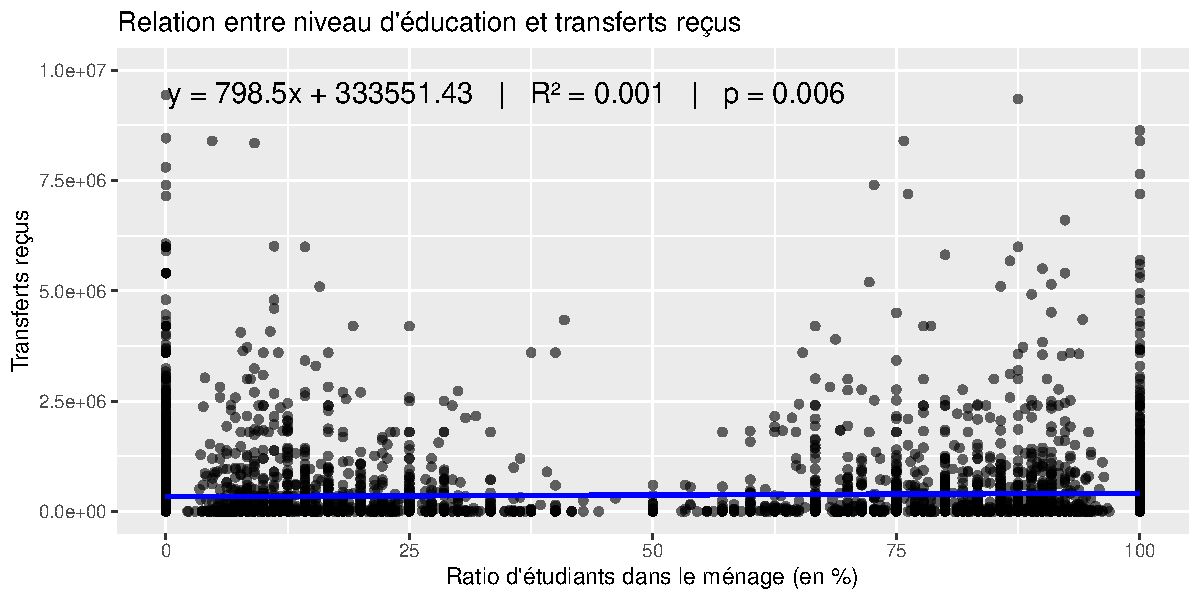
\includegraphics{Beamer_files/figure-beamer/transferts-summary-1.pdf}
\end{frame}

\begin{frame}{1. Analyse de la relation entre les transferts reçus et la
proportion de membres scolarisés au sein des ménages}
\phantomsection\label{analyse-de-la-relation-entre-les-transferts-reuxe7us-et-la-proportion-de-membres-scolarisuxe9s-au-sein-des-muxe9nages-1}
\begin{block}{Interprétation de la regression}
\phantomsection\label{interpruxe9tation-de-la-regression}
La régression linéaire (\(y = 798.5x + 333551.43\)) montre une faible
relation positive entre le niveau d'éducation (ratio d'étudiants par
ménage) et les transferts reçus. Cependant, le \(R^2\) de \textbf{0,001}
révèle que l'éducation explique seulement \textbf{0,1\%} de la variation
des transferts, ce qui est négligeable.

Bien que le résultat soit statistiquement significatif (\(p = 0,006\)),
l'impact pratique est quasi inexistant, suggérant que d'autres facteurs
non mesurés déterminent principalement les transferts.
\end{block}
\end{frame}

\begin{frame}{1. Analyse de la relation entre les transferts reçus et la
proportion de membres scolarisés au sein des ménages}
\phantomsection\label{analyse-de-la-relation-entre-les-transferts-reuxe7us-et-la-proportion-de-membres-scolarisuxe9s-au-sein-des-muxe9nages-2}
Par la suite, suivant la proportion de membres scolarisés au sein des
ménages, nous avons subdivisé les ménages en 04 groupes :

\begin{itemize}
\item
  Faible ({[} 0 \%, 25 \% {[})
\item
  Modéré ({[} 25 \%, 50 \% {[})
\item
  Élevé ({[} 50 \%, 75 \% {[})
\item
  Très élevé ({[} 75 \%, 100 \% {[})
\end{itemize}
\end{frame}

\begin{frame}{1. Analyse de la relation entre les transferts reçus et la
proportion de membres scolarisés au sein des ménages}
\phantomsection\label{analyse-de-la-relation-entre-les-transferts-reuxe7us-et-la-proportion-de-membres-scolarisuxe9s-au-sein-des-muxe9nages-3}
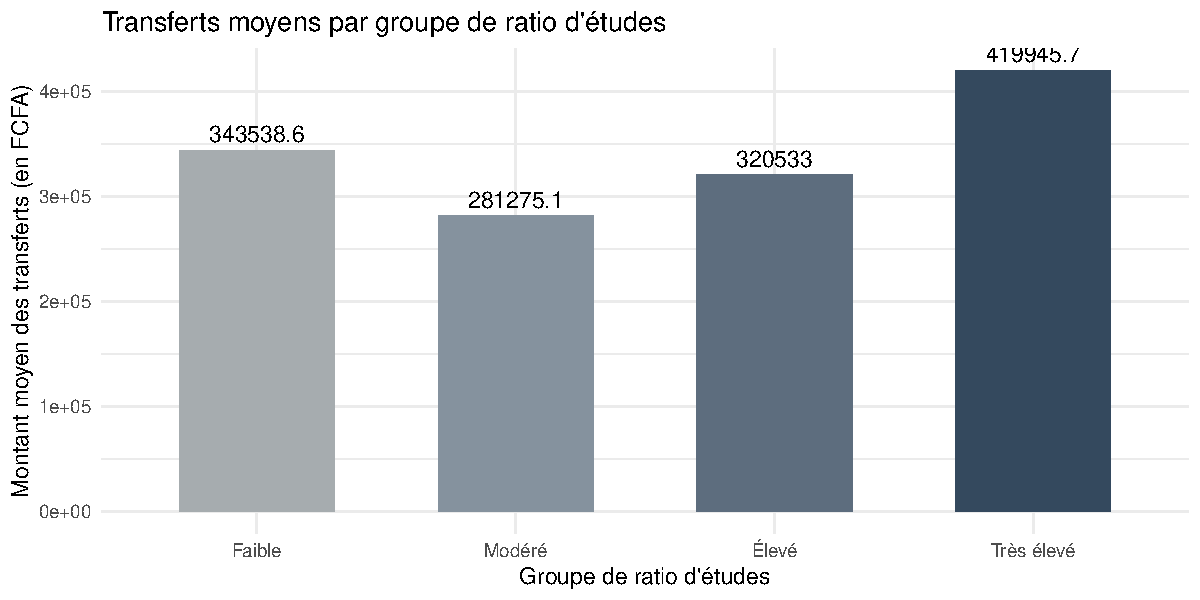
\includegraphics{Beamer_files/figure-beamer/transferts-summary2-1.pdf}
\end{frame}

\begin{frame}{1. Analyse de la relation entre les transferts reçus et la
proportion de membres scolarisés au sein des ménages}
\phantomsection\label{analyse-de-la-relation-entre-les-transferts-reuxe7us-et-la-proportion-de-membres-scolarisuxe9s-au-sein-des-muxe9nages-4}
\begin{block}{Interprétation du graphique}
\phantomsection\label{interpruxe9tation-du-graphique}
Le graphique montre une distribution asymétrique des transferts avec des
valeurs extrêmes atteignant 25 millions FCFA, ce qui distord la
visualisation. Les boîtes à moustaches (boxplots) semblent compressées
en bas du graphique, indiquant que la majorité des transferts se situent
bien en-dessous de 5 millions FCFA pour les quatre groupes de
scolarisation (Faible à Très élevé).
\end{block}
\end{frame}

\begin{frame}[fragile]{2. Analyse de la relation entre les transferts
reçus et les dépenses en santé}
\phantomsection\label{analyse-de-la-relation-entre-les-transferts-reuxe7us-et-les-duxe9penses-en-santuxe9}
\begin{verbatim}
## `geom_smooth()` using formula = 'y ~ x'
\end{verbatim}

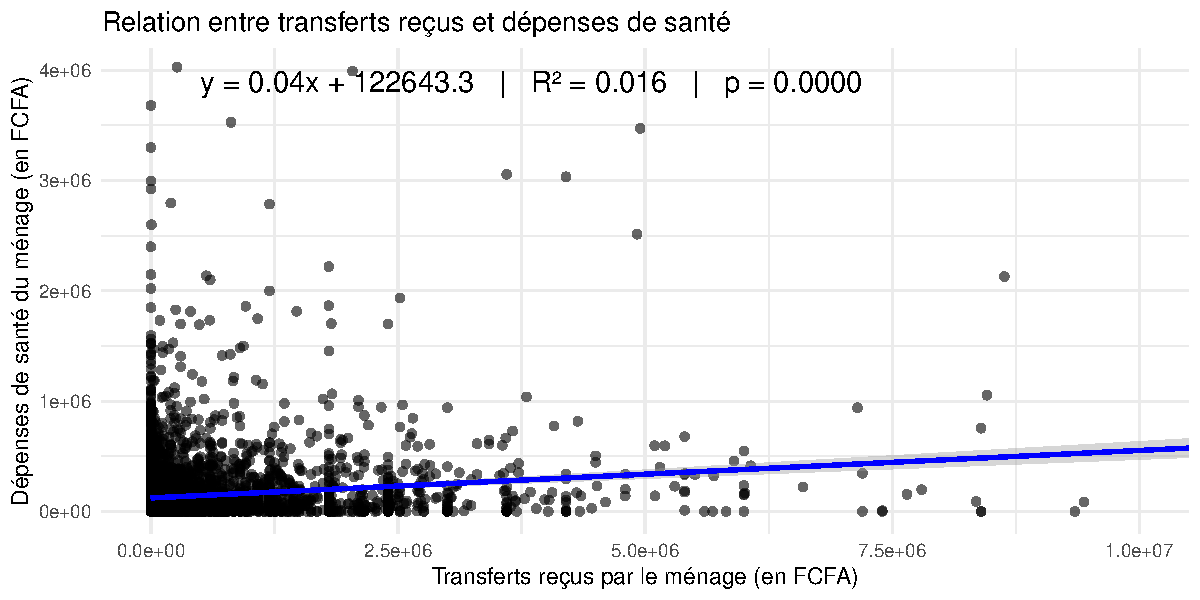
\includegraphics{Beamer_files/figure-beamer/transferts-summary3-1.pdf}
\end{frame}

\begin{frame}{2. Analyse de la relation entre les transferts reçus et
les dépenses en santé}
\phantomsection\label{analyse-de-la-relation-entre-les-transferts-reuxe7us-et-les-duxe9penses-en-santuxe9-1}
\begin{block}{Interprétation de la regression}
\phantomsection\label{interpruxe9tation-de-la-regression-1}
La régression linéaire montre une relation faible mais statistiquement
significative entre les transferts reçus et les dépenses de santé (p
\textless{} 0.001). L'équation y = 0.04x + 122 643 indique qu'une
augmentation de 1 FCFA de transferts est associée à une hausse de 0,04
FCFA des dépenses de santé. Cependant, le R² de 0,016 révèle que
seulement 1,6\% de la variation des dépenses de santé s'explique par les
transferts, suggérant que d'autres facteurs non pris en compte dominent
cette relation. La présence de valeurs extrêmes (jusqu'à 2,5-5 millions
FCFA) visible dans le graphique pourrait influencer ces résultats.
\end{block}
\end{frame}

\begin{frame}{3. Analyse de la relation entre transferts reçus et revenu
total non issu du rendement agricole (emploi, non emploi et transfert)}
\phantomsection\label{analyse-de-la-relation-entre-transferts-reuxe7us-et-revenu-total-non-issu-du-rendement-agricole-emploi-non-emploi-et-transfert}
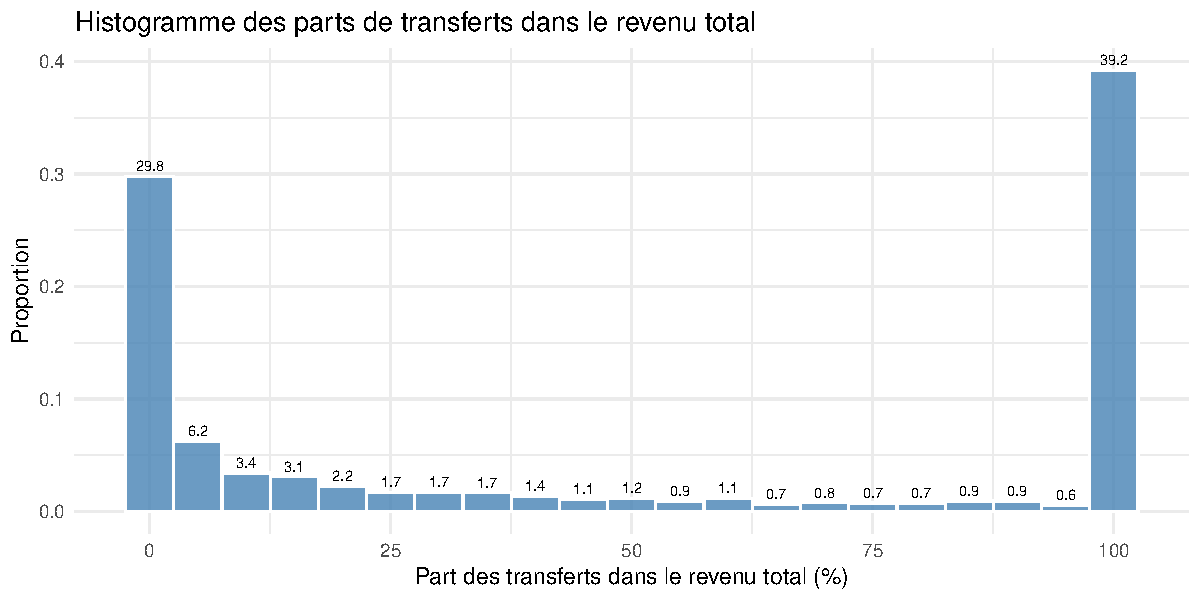
\includegraphics{Beamer_files/figure-beamer/transferts-summary4-1.pdf}
\end{frame}

\begin{frame}{3. Analyse de la relation entre transferts reçus et revenu
total non issu du rendement agricole (emploi,non emploi et transfert)}
\phantomsection\label{analyse-de-la-relation-entre-transferts-reuxe7us-et-revenu-total-non-issu-du-rendement-agricole-emploinon-emploi-et-transfert}
\begin{block}{Interprétation du graphique}
\phantomsection\label{interpruxe9tation-du-graphique-1}
L'histogramme montre une distribution asymétrique des parts de
transferts dans le revenu total, avec deux pics principaux : un premier
pic important à 29,8\% et un second pic plus marqué à 39,2\%. La
majorité des observations se concentrent entre 0,7\% et 3,1\%, mais la
représentation graphique indique que certains ménages dépendent
fortement des transferts. Cette distribution quasi bimodale suggère
l'existence de deux sous-populations distinctes : une proportion
significative pour qui les transferts représentent une part modeste du
revenu (moins de 5\%), et une autre pour qui ils constituent une
ressource essentielle (plus de 50\%), ce qui témoigne de situations de
forte dépendance aux transferts pour certains ménages.
\end{block}
\end{frame}

\begin{frame}[fragile]{3. Analyse de la relation entre transferts reçus
et revenu total non issu du rendement agricole (emploi, non emploi et
transfert)}
\phantomsection\label{analyse-de-la-relation-entre-transferts-reuxe7us-et-revenu-total-non-issu-du-rendement-agricole-emploi-non-emploi-et-transfert-1}
\begin{verbatim}
## `geom_smooth()` using formula = 'y ~ x'
\end{verbatim}

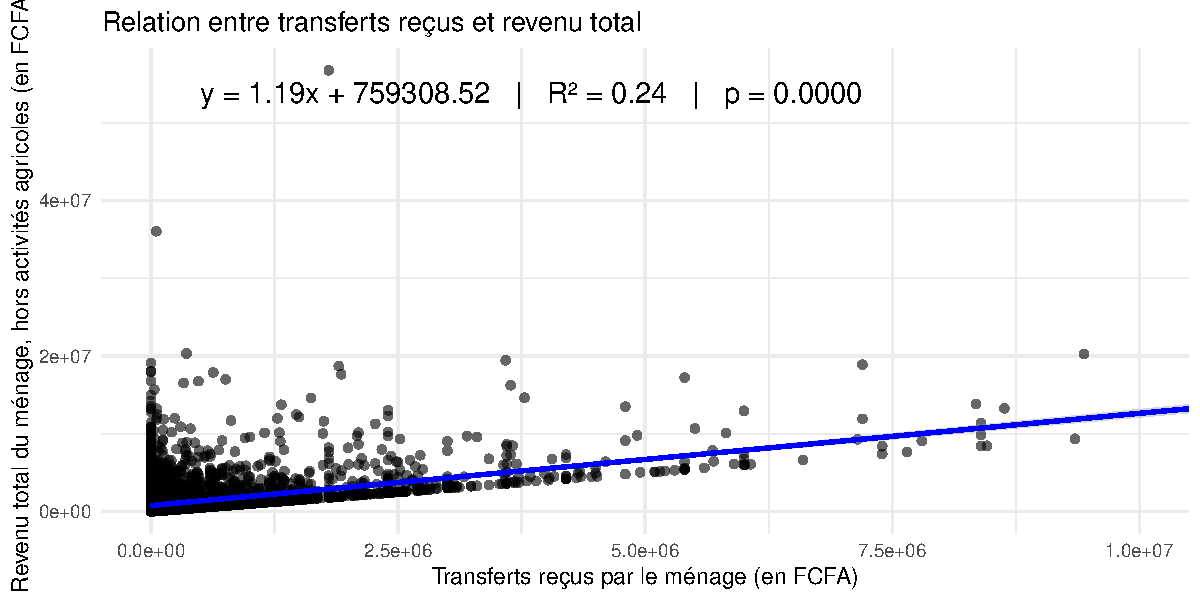
\includegraphics{Beamer_files/figure-beamer/transferts-summary5-1.pdf}
\end{frame}

\begin{frame}{3. Analyse de la relation entre transferts reçus et revenu
total non issu du rendement agricole (emploi, non emploi et transfert)}
\phantomsection\label{analyse-de-la-relation-entre-transferts-reuxe7us-et-revenu-total-non-issu-du-rendement-agricole-emploi-non-emploi-et-transfert-2}
\begin{block}{Interprétation de la regression}
\phantomsection\label{interpruxe9tation-de-la-regression-2}
La régression révèle une relation positive significative (p \textless{}
0,001) entre transferts et revenus, avec un coefficient de 1,19 (chaque
FCFA de revenu supplémentaire étant associé à 1,19 FCFA de transferts en
moyenne). Le R² de 0,24 indique une corrélation modérée, où 24\% de la
variation des transferts s'explique par le revenu.

Cette relation suggère deux mécanismes probables : les ménages aisés
bénéficient de réseaux sociaux plus productifs (transferts privés
accrues des diasporas), et/ou les transferts institutionnels (aides
publiques, ONG) ciblent partiellement les ménages selon leur niveau de
ressources.

La présence de valeurs élevées (jusqu'à 2,5 millions FCFA) montre que
l'effet est particulièrement marqué pour certains ménages, possiblement
urbains ou avec migrants internationaux.
\end{block}
\end{frame}

\section{Limites du projet}\label{limites-du-projet}

\begin{frame}{Limites du projet}
\phantomsection\label{limites-du-projet-1}
\begin{block}{Approche descriptive et corrélationnelle :}
\phantomsection\label{approche-descriptive-et-corruxe9lationnelle}
L'analyse repose principalement sur des statistiques descriptives et des
corrélations, sans recours à des méthodes économétriques avancées
(modèles multivariés, techniques d'identification causale).
\end{block}

\begin{block}{Absence d'interprétation causale :}
\phantomsection\label{absence-dinterpruxe9tation-causale}
Les relations observées entre transferts et bien-être ne peuvent être
interprétées comme des liens de causalité.
\end{block}

\begin{block}{Données transversales :}
\phantomsection\label{donnuxe9es-transversales}
La base EHCVM 2018 étant transversale, elle ne permet pas de suivre les
ménages dans le temps ni de mesurer les effets dynamiques des
transferts.
\end{block}
\end{frame}

\begin{frame}{Limites du projet}
\phantomsection\label{limites-du-projet-2}
\begin{block}{Biais de mesure possibles :}
\phantomsection\label{biais-de-mesure-possibles}
Les revenus et dépenses sont auto-déclarés, ce qui peut introduire des
biais liés à la mémoire, la perception ou la volonté de l'enquêté.
\end{block}

\begin{block}{Indicateurs de bien-être incomplets :}
\phantomsection\label{indicateurs-de-bien-uxeatre-incomplets}
Des dimensions essentielles comme la nutrition, le logement ou l'accès
aux services publics n'ont pas pu être intégrées à l'analyse.
\end{block}

\begin{block}{Typologie éducative simplifiée :}
\phantomsection\label{typologie-uxe9ducative-simplifiuxe9e}
Le ratio d'individus scolarisés utilisé pour classer les ménages reste
une approximation qui ne reflète pas pleinement la complexité des
situations éducatives et socioéconomiques.
\end{block}
\end{frame}

\section{Conclusion}\label{conclusion}

\begin{frame}{Enseignements de l'étude}
\phantomsection\label{enseignements-de-luxe9tude}
\begin{block}{Rôle contrasté des transferts :}
\phantomsection\label{ruxf4le-contrastuxe9-des-transferts}
Les transferts jouent un rôle important mais inégal dans le bien-être
des ménages sénégalais.
\end{block}

\begin{block}{Effets différenciés selon le niveau de scolarisation :}
\phantomsection\label{effets-diffuxe9renciuxe9s-selon-le-niveau-de-scolarisation}
L'impact est plus marqué chez les ménages faiblement et très scolarisés.
\end{block}
\end{frame}

\begin{frame}{Enseignements de l'étude}
\phantomsection\label{enseignements-de-luxe9tude-1}
\begin{block}{Impact limité sur la santé :}
\phantomsection\label{impact-limituxe9-sur-la-santuxe9}
Faible pouvoir explicatif des transferts sur les dépenses de santé (R² =
1,6 \%).
\end{block}

\begin{block}{Effet significatif sur le revenu total :}
\phantomsection\label{effet-significatif-sur-le-revenu-total}
Les transferts expliquent 24 \% de la variance du revenu total,
suggérant un effet multiplicateur.
\end{block}
\end{frame}

\begin{frame}{Recommandations}
\phantomsection\label{recommandations}
\begin{block}{Recommandation 1 : ciblage renforcé}
\phantomsection\label{recommandation-1-ciblage-renforcuxe9}
Utiliser des indicateurs de vulnérabilité pour mieux orienter les
transferts et anticiper les chocs.
\end{block}

\begin{block}{Recommandation 2 : mobilisation de la diaspora}
\phantomsection\label{recommandation-2-mobilisation-de-la-diaspora}
Encourager l'usage de plateformes digitales sécurisées pour accroître
les flux et renforcer l'effet réseau.
\end{block}
\end{frame}

\begin{frame}{Perspectives}
\phantomsection\label{perspectives}
\begin{block}{Vers une stratégie intégrée :}
\phantomsection\label{vers-une-stratuxe9gie-intuxe9gruxe9e}
Une approche combinant protection sociale adaptative et inclusion
financière renforcerait la résilience face aux chocs climatiques et
économiques, tout en réduisant les inégalités.
\end{block}
\end{frame}

\end{document}
